\documentclass[11pt]{article}
\usepackage[utf8]{inputenc}
\usepackage[margin=3cm]{geometry}
\usepackage{amsmath}
\usepackage[style=authoryear, citestyle=authoryear]{biblatex}
\usepackage[colorlinks=true, citecolor=blue, linkcolor=blue, hyperfootnotes=false]{hyperref} 
\usepackage[multiple]{footmisc}
\usepackage{graphicx}
\usepackage[font=footnotesize, labelfont=bf]{caption}

\title{CTA200H Computing Assignment}
\author{Mathew Bub \\ Supervisor: Cristobal Petrovich}
\date{May 17, 2019}

\newcommand{\evec}{\mathbf{e}}
\newcommand{\ehat}{\hat{\evec}}
\newcommand{\jvec}{\mathbf{j}}
\newcommand{\jhat}{\hat{\jvec}}
\newcommand{\Jvec}{\mathbf{J}}
\newcommand{\rpl}{\mathbf{r_{\mathrm{pl}}}}
\newcommand{\rplhat}{\mathbf{\hat{r}_{\mathrm{pl}}}}
\newcommand{\xvec}{\mathbf{x}}

\addbibresource{refs.bib}

\begin{document}

\maketitle

\section*{Introduction}
This assignment studies the evolution of a binary system under the influence of the tidal field of a distant third body. In this case, we study the evolution of the orbit of the Moon under the effect of the tidal field of the Sun.

Here, we will use vectorial formalism \parencite{tremaine2014} to describe the orbits under study, rather than the more traditional orbital elements. Under the vectorial formalism, we define an orthonormal basis $\{\ehat, \jhat \times \ehat, \jhat\}$, where $\ehat$ points in the direction of the pericentre of the Moon's orbit, and $\jhat$ points in the direction of the angular momentum $\Jvec$. Then, the shape of the Moon's orbit is described by
\begin{align}
    \evec &= e \, \ehat \label{eq:evec} \\
    \jvec &= \sqrt{1-e^2} \, \jhat \label{eq:jvec}
\end{align}
where $e$ is the eccentricity of the orbit. 

\section*{Part 1: The Evolution of Moons Around Planets}
Assuming that the Moon is massless, then according to the assignment sheet and the accompanying notes by Antognini, the secular evolution for the Moon perturbed by the Sun reads
\begin{align}
    \frac{d\evec}{dt} &= -\tau_{\mathrm{moon}}^{-1}[2 \jvec \times \evec - 5(\rplhat \cdot \evec) \jvec \times \rplhat + (\rplhat \cdot \jvec) \evec \times \rplhat] \label{eq:devec} \\
    \frac{d\jvec}{dt} &= -\tau_{\mathrm{moon}}^{-1}[(\rplhat \cdot \jvec) \jvec \times \rplhat - 5(\rplhat \cdot \evec) \evec \times \rplhat] \label{eq:djvec}
\end{align}
where $\rpl$ is the position of the Earth in its orbit about the Sun, which is assumed to be circular and is therefore given by
\begin{equation} \label{eq:rpl}
    \rpl(t) = 1 \, \mathrm{AU} \, (\cos(2 \pi t/1 \, \mathrm{year}), \; \sin(2 \pi t/1 \, \mathrm{year}), \; 0)
\end{equation}
and
\begin{equation} \label{eq:tau}
    \tau_{\mathrm{moon}} = \frac{m_{\mathrm{earth}}}{m_{\mathrm{sun}}} \frac{r_{\mathrm{pl}}(t)^3}{a_{\mathrm{moon}}^3} \frac{P_{\mathrm{moon}}}{3 \pi}.
\end{equation}
By Kepler's third law, we also have that
\begin{equation} \label{eq:Pmoon}
    P_{\mathrm{moon}} = 2\pi \left( \frac{a_{\mathrm{moon}}^3}{Gm_{\mathrm{earth}}} \right)^{1/2}.
\end{equation}

Using this, we can calculate $\tau_{\mathrm{moon}}$ for the current separation of the Moon. Working in units of AU/$M_\odot$/yr, we have that\footnote{\url{https://en.wikipedia.org/wiki/Gravitational\_constant}}\footnote{\url{https://en.wikipedia.org/wiki/Earth\_mass}}\footnote{\url{https://en.wikipedia.org/wiki/Lunar\_distance\_(astronomy)}}
\begin{align*}
    G &\approx 4 \pi^2 \; \mathrm{AU}^3 \: \mathrm{yr}^{-2} \: M_\odot^{-1} \\
    m_{\mathrm{earth}} &= 3.003 \times 10^{-6} \; M_\odot \\
    a_{\mathrm{moon}} &= 1/388.6 \; \mathrm{AU}.
\end{align*}
Substituting these into (\ref{eq:tau}) gives (see the accompanying Python script)
\[
    \tau_{\mathrm{moon}} = 1.409 \; \mathrm{yr}.
\]
If instead we assume that the Moon is 10 times closer than its current separation, we find that
\[
    \tau_{\mathrm{moon}} = 44.54 \; \mathrm{yr}.
\]

We now implement a $4^\mathrm{th}$ order Runge-Kutta (RK4) integrator to evolve equations (\ref{eq:devec}) and (\ref{eq:djvec}). In general, given a system of ordinary differential equations $\xvec' = \mathbf{F}(\xvec, t)$ and initial data $\xvec(t)$, we can compute $\xvec(t + \Delta t)$ using the RK4 method according to the formula
\begin{equation} \label{eq:RK4}
    \xvec(t + \Delta t) = \xvec(t) + \frac{\mathbf{m} + 2\mathbf{n} + 2\mathbf{p} + \mathbf{q}}{6} \Delta t
\end{equation}
where
\begin{align}
\begin{split} \label{eq:RK4_derivatives}
    \mathbf{m} &= \mathbf{F} \left( \xvec, t \right) \\
    \mathbf{n} &= \mathbf{F} \left( \xvec + \textbf{m} \cdot \tfrac{1}{2} \Delta t, t + \tfrac{1}{2} \Delta t \right) \\
    \mathbf{p} &= \mathbf{F} \left( \xvec + \textbf{n} \cdot \tfrac{1}{2} \Delta t, t + \tfrac{1}{2} \Delta t \right) \\
    \mathbf{q} &= \mathbf{F} \left( \xvec + \textbf{p} \cdot \Delta t, t + \Delta t \right)
\end{split}
\end{align}
\parencite{hirsch2013}. For our integration, we use the following initial conditions:
\begin{itemize}
    \item Longitude of the ascending node: $\Omega = 0$
    \item Argument of the pericentre: $\omega = 90^\circ$
    \item Inclination: $I = 60^\circ$
    \item Eccentricity: $e = 0.05$.
\end{itemize}
From these initial conditions, we compute the initial values of $\evec$ and $\jvec$ according to the identities
\begin{align}
    \evec(t=0) &= e_0 [\cos \omega \cos \Omega - \sin \omega \sin \Omega \cos I, \cos \omega \sin \Omega + \sin \omega \cos \Omega \cos I, \sin I \sin \omega] \label{evec_elements} \\
    \jvec(t=0) &= \sqrt{1 - e_0^2}[\sin I \sin \Omega, -\sin I \cos \Omega, \cos I] \label{jvec_elements}.
\end{align}
We then integrate equations (\ref{eq:devec}) and (\ref{eq:djvec}) forward for $10 \tau_\mathrm{moon}$, using a fixed time step size of $\Delta t = 1/20 \; \mathrm{yr}$. We perform this integration twice, using both $\tau_{\mathrm{moon}} = 1.409 \; \mathrm{yr}$ and $\tau_{\mathrm{moon}} = 44.54 \; \mathrm{yr}$. Sanity checks confirm that the equations preserve the orthogonality ($\evec \cdot \jvec = 0$) and the norm ($|\evec|^2 + |\jvec|^2 = 1)$ of the vector elements to within an error of approximately $10^{-5}$.

\section*{Part 2: Plotting the Orbital Elements}
After completing the RK4 integration, we convert the $\evec$ and $\jvec$ vectors to the classical orbital elements using the identities
\begin{align}
    I &= \arctan \left( \sqrt{j_x^2 + j_y^2} / j_z \right) \label{eq:I} \\
    \Omega &= \arctan(-j_x / j_y) \label{eq:Omega} \\
    \omega &= \arctan \left( \frac{-e_x \sin \Omega + e_y \cos \Omega \cos I + e_z \sin I}{e_x \cos \Omega + e_y \sin \Omega} \right) \label{eq:omega}.
\end{align}
Figure \ref{fig:panels} shows plots of these orbital elements over the integration period in the case where $\tau_{\mathrm{moon}} = 1.409 \; \mathrm{yr}$. In each of the panels, two distinct oscillatory patterns are visible. The stronger and lower frequency oscillations correspond to Lidov-Kozai cycles, similar to those originating from the doubly-averaged lunar potential of \textcite{tremaine2014}. The smaller, higher frequency oscillations correspond to deviations from the doubly-averaged potential, and as such have a timescale similar to the orbital period of the Earth. In panel \textbf{(a)}, we have also marked the position of the predicted maximum eccentricity achieved in the Lidov-Kozai cycles of a satellite with initial inclination $I_0$. This value is $e_\mathrm{max} = \sqrt{1 - \tfrac{5}{3} \cos^2 I_0}$. Evidently, this predicted maximum agrees with the maximum achieved during the integration. Finally, note that $j_z$ is not conserved except in an average sense, due to the shorter-scale oscillations relating to the orbit of the Earth.

\begin{figure}[h!]
    \centering
    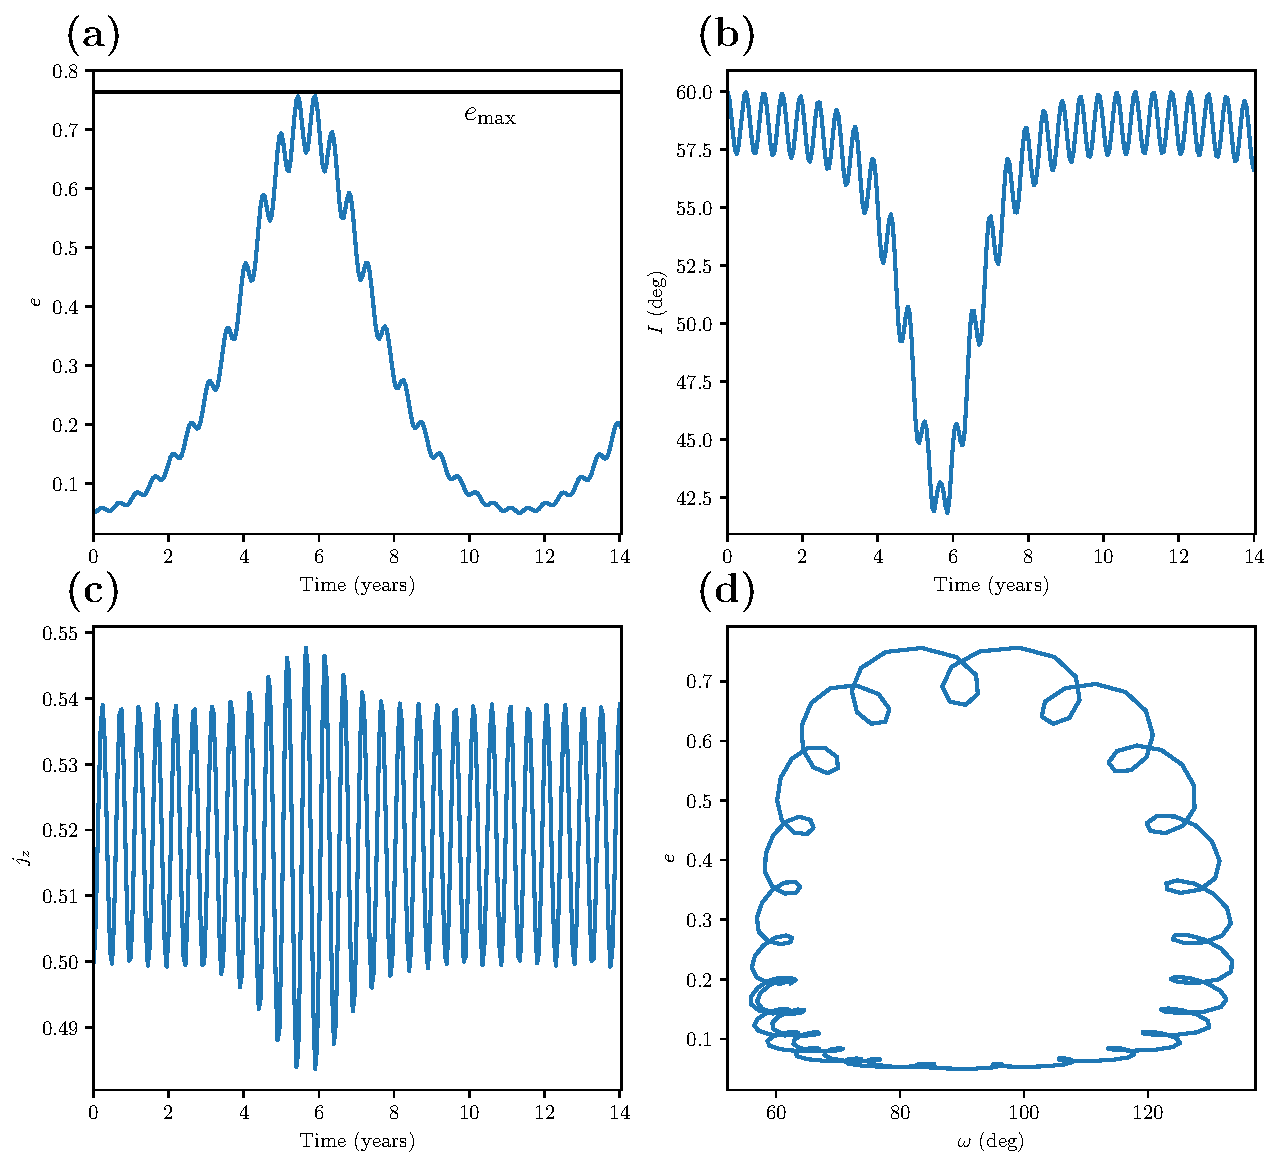
\includegraphics[width=\textwidth]{plots/figure1.pdf}
    \caption{Results of the RK4 integration using $\tau_\mathrm{moon} = 1.409 \; \mathrm{yr}$. \textbf{(a)} $e$ as a function of time. The larger oscillations correspond to Lidov-Kozai cycles, while the smaller oscillations correspond to deviations from these cycles on the timescale of the Earth's orbital period. The black line corresponds to the predicted maximum eccentricity of the Lidov-Kozai cycles, $e_\mathrm{max} = \sqrt{1 - \tfrac{5}{3} \cos^2 I_0}$. \textbf{(b)} $I$ as a function of time. \textbf{(c)} $j_z = \sqrt{1-e^2} \cos I$ as a function of time. Note that $j_z$ is not conserved on the timescale of the Earth's orbital period, but is conserved on average on the timescale of the Lidov-Kozai oscillations. \textbf{(d)} $e$ vs. $\omega$.}
    \label{fig:panels}
\end{figure}

Figure \ref{fig:panels_close} shows the same orbital element plots as previously, now in the case where $\tau_{\mathrm{moon}} = 44.54 \; \mathrm{yr}$. Since $\tau_\mathrm{moon} \gg 1 \; \mathrm{yr}$ in this case, the Lidov-Kozai oscillations now dominate, and the higher-frequency oscillations are marginal. Moreover, $j_z$ is now closer to being conserved, as can be seen in panel \textbf{(c)}, where the oscillations are of a smaller magnitude than those of Figure \ref{fig:panels}. Thus, the results using the larger value of $\tau_{\mathrm{moon}}$ are in closer agreement with the doubly-averaged lunar potential of \textcite{tremaine2014} than previously, reflecting that the orbital period of the Earth is less significant at this larger timescale.

\begin{figure}[h!]
    \centering
    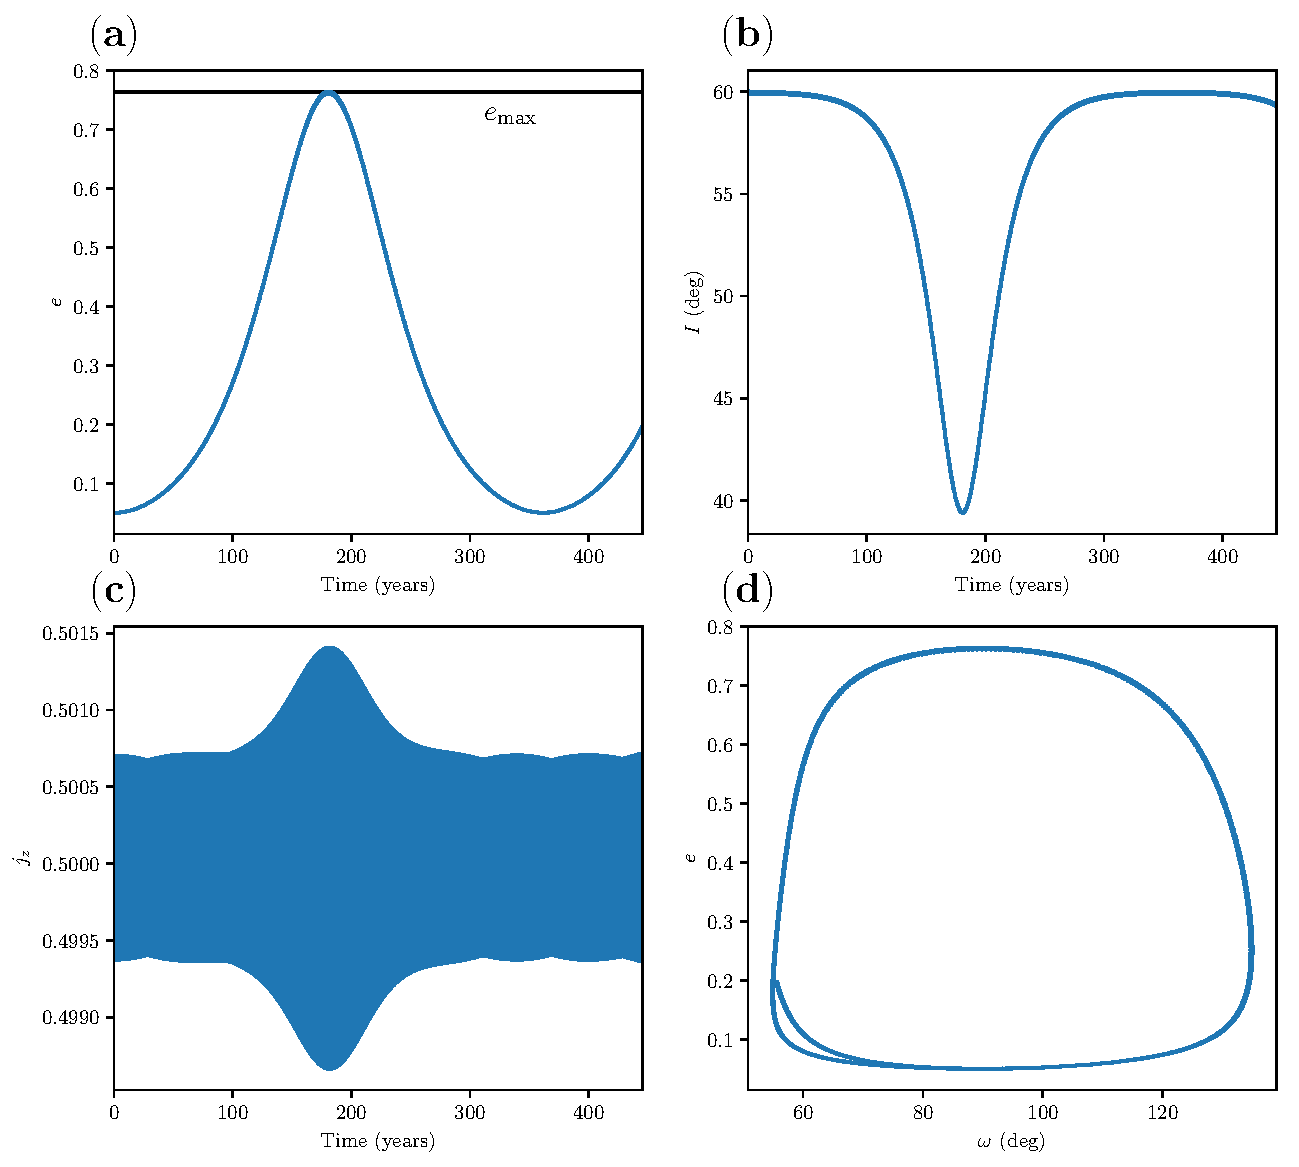
\includegraphics[width=\textwidth]{plots/figure2.pdf}
    \caption{Results of the RK4 integration using $\tau_\mathrm{moon} = 44.54 \; \mathrm{yr}$. \textbf{(a)} $e$ as a function of time. Notice that the Lidov-Kozai oscillations now dominate with the larger timescale, in contrast to Figure \ref{fig:panels}, where the timescale of the Earth's orbit is still significant. \textbf{(b)} $I$ as a function of time. \textbf{(c)}  $j_z = \sqrt{1-e^2} \cos I$ as a function of time. The plot appears to be a solid colour because the frequency of the smaller oscillations is much larger than the frequency of the Lidov-Kozai oscillations. Notice that the magnitude of the oscillations here are significantly smaller than those of Figure \ref{fig:panels}, indicating that $j_z$ is closer to being conserved. \textbf{(d)} $e$ vs. $\omega$.}
    \label{fig:panels_close}
\end{figure}

\section*{Part 3: A Colliding Moon}
Figure \ref{fig:e_max} show $e$ as a function of time for $I_0 = 30^\circ$, $45^\circ$, and $80^\circ$, using $\tau_\mathrm{moon} = 44.54 \; \mathrm{yr}$. We are using the larger value of $\tau_\mathrm{moon}$ here to ensure that each cycle is dominated by the Lidov-Kozai cycle, thereby reaching the predicted maximum eccentricity, $e_\mathrm{max} = \sqrt{1 - \tfrac{5}{3} \cos^2 I_0}$. Note that $e_\mathrm{max}$ is not marked for $I_0 = 30^\circ$, since in this case $\tfrac{5}{3} \cos^2 I_0 > 1$.

From this figure, we can see that the period of the Lidov-Kozai cycles appear to increase with decreasing initial inclination. This makes sense, as we would expect the cycles to disappear entirely for $I_0 = 0^\circ$. Moreover, as per the predicted values of $e_\mathrm{max}$, the maximum eccentricity achieved in each cycle increases with initial inclination. In particular, an initial inclination of $I_0 = 80^\circ$ leads to a collision with the Earth, as indicated by the horizontal red line. Thus, the perturbations due to the Sun cause highly inclined orbits to be unstable.

\begin{figure}[h!]
    \centering
    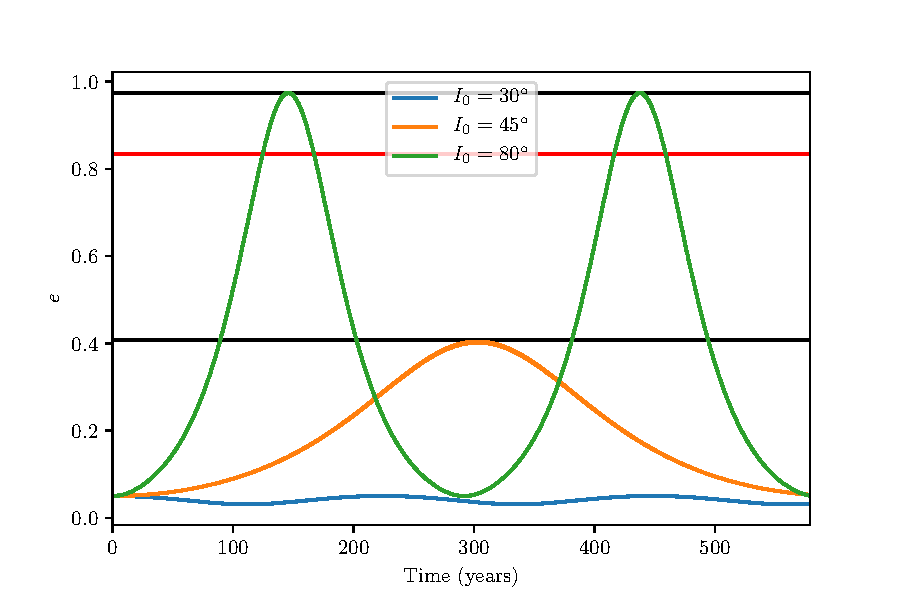
\includegraphics[width=\textwidth]{plots/figure3.pdf}
    \caption{$e$ as a function of time using various initial inclinations and $\tau_\mathrm{moon} = 44.54 \; \mathrm{yr}$. The black horizontal lines indicate the predicted maximum eccentricity achieved during each Lidov-Kozai cycle, $e_\mathrm{max} = \sqrt{1 - \tfrac{5}{3} \cos^2 I_0}$. The red horizontal line indicates the eccentricity at which the Moon would collide with the Earth, such that $a_\mathrm{moon}(1 - e) = R_\mathrm{earth}$.}
    \label{fig:e_max}
\end{figure}

\section*{Part 4: Testing Different Step Sizes}
Figure \ref{fig:steps} shows $e$ as a function of time using $\tau_{\mathrm{moon}} = 1.409 \; \mathrm{yr}$ and a variety of integrator time step sizes. Here, the curves using $\Delta t = 1/20 \; \mathrm{yr}$ and $\Delta t = 1/10 \; \mathrm{yr}$ follow each other reasonably closely for the entire integration period. The curve using  $\Delta t = 1/5 \; \mathrm{yr}$ roughly follows the shape of the previous two curves for most of the integration time, but begins to diverge toward the end of the integration. From this, we may conclude that in order to ensure an accurate approximation of the dynamical evolution of a system, the integrator must use a time step size significantly smaller than the shortest time scale in the problem (in this case, the orbital period of the Earth, 1 year). This constraint can become cumbersome when one's largest timescale is significantly larger than one's shortest timescale (for instance, the orbital period of a compact binary versus its orbital period in the Galaxy). Thus, the technique of orbit-averaging allows us to ignore some of the shorter timescales, thereby allowing us to use larger time steps.

\begin{figure}[h!]
    \centering
    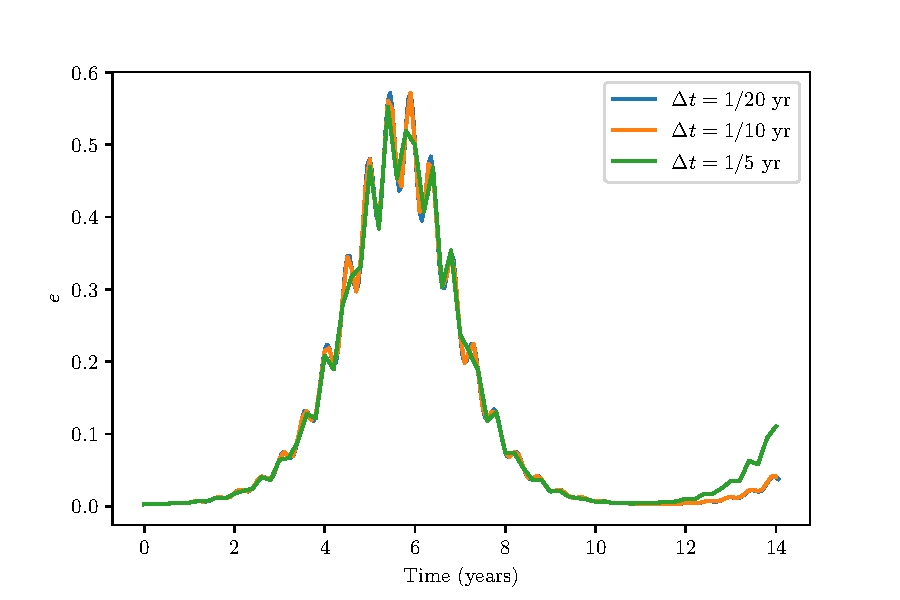
\includegraphics[width=\textwidth]{plots/figure4.pdf}
    \caption{$e$ as a function of time using various time step sizes and $\tau_{\mathrm{moon}} = 1.409 \; \mathrm{yr}$.}
    \label{fig:steps}
\end{figure}

\section*{Conclusions}
In this assignment, we investigated the effect of the Sun perturbing the orbit of the Moon using vectorial formalism, orbit-averaging techniques, and a $4^\mathrm{th}$ order Runge-Kutta integrator. Here, we examined the appearance of Lidov-Kozai oscillations, which cause oscillations in the eccentricity and inclination of the Moon's orbit while keeping $j_z$ approximately constant. The magnitude of these oscillations was found to be dependent on the initial inclination, with high inclinations leading to a collision of the Moon and the Earth. We also examined how these oscillations are affected by the timescale of the problem. In particular, we considered how the orbit of the Moon deviates from Lidov-Kozai oscillations on the timescale of the orbit of the Earth. Finally, we discussed how the quality of the numerical integration is affected by the step size of the integrator. These investigations will serve as a useful primer to applying similar techniques to the evolution of binary systems near the Galactic centre.

\printbibliography
\end{document}
